
%% bare_jrnl.tex
%% V1.3
%% 2007/01/11
%% by Michael Shell
%% see http://www.michaelshell.org/
%% for current contact information.
%%
%% This is a skeleton file demonstrating the use of IEEEtran.cls
%% (requires IEEEtran.cls version 1.7 or later) with an IEEE journal paper.
%%
%% Support sites:
%% http://www.michaelshell.org/tex/ieeetran/
%% http://www.ctan.org/tex-archive/macros/latex/contrib/IEEEtran/
%% and
%% http://www.ieee.org/



% *** Authors should verify (and, if needed, correct) their LaTeX system  ***
% *** with the testflow diagnostic prior to trusting their LaTeX platform ***
% *** with production work. IEEE's font choices can trigger bugs that do  ***
% *** not appear when using other class files.                            ***
% The testflow support page is at:
% http://www.michaelshell.org/tex/testflow/


%%*************************************************************************
%% Legal Notice:
%% This code is offered as-is without any warranty either expressed or
%% implied; without even the implied warranty of MERCHANTABILITY or
%% FITNESS FOR A PARTICULAR PURPOSE! 
%% User assumes all risk.
%% In no event shall IEEE or any contributor to this code be liable for
%% any damages or losses, including, but not limited to, incidental,
%% consequential, or any other damages, resulting from the use or misuse
%% of any information contained here.
%%
%% All comments are the opinions of their respective authors and are not
%% necessarily endorsed by the IEEE.
%%
%% This work is distributed under the LaTeX Project Public License (LPPL)
%% ( http://www.latex-project.org/ ) version 1.3, and may be freely used,
%% distributed and modified. A copy of the LPPL, version 1.3, is included
%% in the base LaTeX documentation of all distributions of LaTeX released
%% 2003/12/01 or later.
%% Retain all contribution notices and credits.
%% ** Modified files should be clearly indicated as such, including  **
%% ** renaming them and changing author support contact information. **
%%
%% File list of work: IEEEtran.cls, IEEEtran_HOWTO.pdf, bare_adv.tex,
%%                    bare_conf.tex, bare_jrnl.tex, bare_jrnl_compsoc.tex
%%*************************************************************************

% Note that the a4paper option is mainly intended so that authors in
% countries using A4 can easily print to A4 and see how their papers will
% look in print - the typesetting of the document will not typically be
% affected with changes in paper size (but the bottom and side margins will).
% Use the testflow package mentioned above to verify correct handling of
% both paper sizes by the user's LaTeX system.
%
% Also note that the "draftcls" or "draftclsnofoot", not "draft", option
% should be used if it is desired that the figures are to be displayed in
% draft mode.
%
\documentclass[journal]{IEEEtran}
\usepackage{blindtext}
\usepackage{graphicx}
\usepackage{verbatim}
\usepackage{caption}
\usepackage{subfigure}

% Some very useful LaTeX packages include:
% (uncomment the ones you want to load)


% *** MISC UTILITY PACKAGES ***
%
%\usepackage{ifpdf}
% Heiko Oberdiek's ifpdf.sty is very useful if you need conditional
% compilation based on whether the output is pdf or dvi.
% usage:
% \ifpdf
%   % pdf code
% \else
%   % dvi code
% \fi
% The latest version of ifpdf.sty can be obtained from:
% http://www.ctan.org/tex-archive/macros/latex/contrib/oberdiek/
% Also, note that IEEEtran.cls V1.7 and later provides a builtin
% \ifCLASSINFOpdf conditional that works the same way.
% When switching from latex to pdflatex and vice-versa, the compiler may
% have to be run twice to clear warning/error messages.






% *** CITATION PACKAGES ***
%
%\usepackage{cite}
% cite.sty was written by Donald Arseneau
% V1.6 and later of IEEEtran pre-defines the format of the cite.sty package
% \cite{} output to follow that of IEEE. Loading the cite package will
% result in citation numbers being automatically sorted and properly
% "compressed/ranged". e.g., [1], [9], [2], [7], [5], [6] without using
% cite.sty will become [1], [2], [5]--[7], [9] using cite.sty. cite.sty's
% \cite will automatically add leading space, if needed. Use cite.sty's
% noadjust option (cite.sty V3.8 and later) if you want to turn this off.
% cite.sty is already installed on most LaTeX systems. Be sure and use
% version 4.0 (2003-05-27) and later if using hyperref.sty. cite.sty does
% not currently provide for hyperlinked citations.
% The latest version can be obtained at:
% http://www.ctan.org/tex-archive/macros/latex/contrib/cite/
% The documentation is contained in the cite.sty file itself.






% *** GRAPHICS RELATED PACKAGES ***
%
\ifCLASSINFOpdf
  % \usepackage[pdftex]{graphicx}
  % declare the path(s) where your graphic files are
  % \graphicspath{{../pdf/}{../jpeg/}}
  % and their extensions so you won't have to specify these with
  % every instance of \includegraphics
  % \DeclareGraphicsExtensions{.pdf,.jpeg,.png}
\else
  % or other class option (dvipsone, dvipdf, if not using dvips). graphicx
  % will default to the driver specified in the system graphics.cfg if no
  % driver is specified.
  % \usepackage[dvips]{graphicx}
  % declare the path(s) where your graphic files are
  % \graphicspath{{../eps/}}
  % and their extensions so you won't have to specify these with
  % every instance of \includegraphics
  % \DeclareGraphicsExtensions{.eps}
\fi
% graphicx was written by David Carlisle and Sebastian Rahtz. It is
% required if you want graphics, photos, etc. graphicx.sty is already
% installed on most LaTeX systems. The latest version and documentation can
% be obtained at: 
% http://www.ctan.org/tex-archive/macros/latex/required/graphics/
% Another good source of documentation is "Using Imported Graphics in
% LaTeX2e" by Keith Reckdahl which can be found as epslatex.ps or
% epslatex.pdf at: http://www.ctan.org/tex-archive/info/
%
% latex, and pdflatex in dvi mode, support graphics in encapsulated
% postscript (.eps) format. pdflatex in pdf mode supports graphics
% in .pdf, .jpeg, .png and .mps (metapost) formats. Users should ensure
% that all non-photo figures use a vector format (.eps, .pdf, .mps) and
% not a bitmapped formats (.jpeg, .png). IEEE frowns on bitmapped formats
% which can result in "jaggedy"/blurry rendering of lines and letters as
% well as large increases in file sizes.
%
% You can find documentation about the pdfTeX application at:
% http://www.tug.org/applications/pdftex





% *** MATH PACKAGES ***
%
%\usepackage[cmex10]{amsmath}
% A popular package from the American Mathematical Society that provides
% many useful and powerful commands for dealing with mathematics. If using
% it, be sure to load this package with the cmex10 option to ensure that
% only type 1 fonts will utilized at all point sizes. Without this option,
% it is possible that some math symbols, particularly those within
% footnotes, will be rendered in bitmap form which will result in a
% document that can not be IEEE Xplore compliant!
%
% Also, note that the amsmath package sets \interdisplaylinepenalty to 10000
% thus preventing page breaks from occurring within multiline equations. Use:
%\interdisplaylinepenalty=2500
% after loading amsmath to restore such page breaks as IEEEtran.cls normally
% does. amsmath.sty is already installed on most LaTeX systems. The latest
% version and documentation can be obtained at:
% http://www.ctan.org/tex-archive/macros/latex/required/amslatex/math/





% *** SPECIALIZED LIST PACKAGES ***
%
%\usepackage{algorithmic}
% algorithmic.sty was written by Peter Williams and Rogerio Brito.
% This package provides an algorithmic environment fo describing algorithms.
% You can use the algorithmic environment in-text or within a figure
% environment to provide for a floating algorithm. Do NOT use the algorithm
% floating environment provided by algorithm.sty (by the same authors) or
% algorithm2e.sty (by Christophe Fiorio) as IEEE does not use dedicated
% algorithm float types and packages that provide these will not provide
% correct IEEE style captions. The latest version and documentation of
% algorithmic.sty can be obtained at:
% http://www.ctan.org/tex-archive/macros/latex/contrib/algorithms/
% There is also a support site at:
% http://algorithms.berlios.de/index.html
% Also of interest may be the (relatively newer and more customizable)
% algorithmicx.sty package by Szasz Janos:
% http://www.ctan.org/tex-archive/macros/latex/contrib/algorithmicx/




% *** ALIGNMENT PACKAGES ***
%
%\usepackage{array}
% Frank Mittelbach's and David Carlisle's array.sty patches and improves
% the standard LaTeX2e array and tabular environments to provide better
% appearance and additional user controls. As the default LaTeX2e table
% generation code is lacking to the point of almost being broken with
% respect to the quality of the end results, all users are strongly
% advised to use an enhanced (at the very least that provided by array.sty)
% set of table tools. array.sty is already installed on most systems. The
% latest version and documentation can be obtained at:
% http://www.ctan.org/tex-archive/macros/latex/required/tools/


%\usepackage{mdwmath}
%\usepackage{mdwtab}
% Also highly recommended is Mark Wooding's extremely powerful MDW tools,
% especially mdwmath.sty and mdwtab.sty which are used to format equations
% and tables, respectively. The MDWtools set is already installed on most
% LaTeX systems. The lastest version and documentation is available at:
% http://www.ctan.org/tex-archive/macros/latex/contrib/mdwtools/


% IEEEtran contains the IEEEeqnarray family of commands that can be used to
% generate multiline equations as well as matrices, tables, etc., of high
% quality.


%\usepackage{eqparbox}
% Also of notable interest is Scott Pakin's eqparbox package for creating
% (automatically sized) equal width boxes - aka "natural width parboxes".
% Available at:
% http://www.ctan.org/tex-archive/macros/latex/contrib/eqparbox/





% *** SUBFIGURE PACKAGES ***
%\usepackage[tight,footnotesize]{subfigure}
% subfigure.sty was written by Steven Douglas Cochran. This package makes it
% easy to put subfigures in your figures. e.g., "Figure 1a and 1b". For IEEE
% work, it is a good idea to load it with the tight package option to reduce
% the amount of white space around the subfigures. subfigure.sty is already
% installed on most LaTeX systems. The latest version and documentation can
% be obtained at:
% http://www.ctan.org/tex-archive/obsolete/macros/latex/contrib/subfigure/
% subfigure.sty has been superceeded by subfig.sty.



%\usepackage[caption=false]{caption}
%\usepackage[font=footnotesize]{subfig}
% subfig.sty, also written by Steven Douglas Cochran, is the modern
% replacement for subfigure.sty. However, subfig.sty requires and
% automatically loads Axel Sommerfeldt's caption.sty which will override
% IEEEtran.cls handling of captions and this will result in nonIEEE style
% figure/table captions. To prevent this problem, be sure and preload
% caption.sty with its "caption=false" package option. This is will preserve
% IEEEtran.cls handing of captions. Version 1.3 (2005/06/28) and later 
% (recommended due to many improvements over 1.2) of subfig.sty supports
% the caption=false option directly:
%\usepackage[caption=false,font=footnotesize]{subfig}
%
% The latest version and documentation can be obtained at:
% http://www.ctan.org/tex-archive/macros/latex/contrib/subfig/
% The latest version and documentation of caption.sty can be obtained at:
% http://www.ctan.org/tex-archive/macros/latex/contrib/caption/




% *** FLOAT PACKAGES ***
%
%\usepackage{fixltx2e}
% fixltx2e, the successor to the earlier fix2col.sty, was written by
% Frank Mittelbach and David Carlisle. This package corrects a few problems
% in the LaTeX2e kernel, the most notable of which is that in current
% LaTeX2e releases, the ordering of single and double column floats is not
% guaranteed to be preserved. Thus, an unpatched LaTeX2e can allow a
% single column figure to be placed prior to an earlier double column
% figure. The latest version and documentation can be found at:
% http://www.ctan.org/tex-archive/macros/latex/base/



%\usepackage{stfloats}
% stfloats.sty was written by Sigitas Tolusis. This package gives LaTeX2e
% the ability to do double column floats at the bottom of the page as well
% as the top. (e.g., "\begin{figure*}[!b]" is not normally possible in
% LaTeX2e). It also provides a command:
%\fnbelowfloat
% to enable the placement of footnotes below bottom floats (the standard
% LaTeX2e kernel puts them above bottom floats). This is an invasive package
% which rewrites many portions of the LaTeX2e float routines. It may not work
% with other packages that modify the LaTeX2e float routines. The latest
% version and documentation can be obtained at:
% http://www.ctan.org/tex-archive/macros/latex/contrib/sttools/
% Documentation is contained in the stfloats.sty comments as well as in the
% presfull.pdf file. Do not use the stfloats baselinefloat ability as IEEE
% does not allow \baselineskip to stretch. Authors submitting work to the
% IEEE should note that IEEE rarely uses double column equations and
% that authors should try to avoid such use. Do not be tempted to use the
% cuted.sty or midfloat.sty packages (also by Sigitas Tolusis) as IEEE does
% not format its papers in such ways.


%\ifCLASSOPTIONcaptionsoff
%  \usepackage[nomarkers]{endfloat}
% \let\MYoriglatexcaption\caption
% \renewcommand{\caption}[2][\relax]{\MYoriglatexcaption[#2]{#2}}
%\fi
% endfloat.sty was written by James Darrell McCauley and Jeff Goldberg.
% This package may be useful when used in conjunction with IEEEtran.cls'
% captionsoff option. Some IEEE journals/societies require that submissions
% have lists of figures/tables at the end of the paper and that
% figures/tables without any captions are placed on a page by themselves at
% the end of the document. If needed, the draftcls IEEEtran class option or
% \CLASSINPUTbaselinestretch interface can be used to increase the line
% spacing as well. Be sure and use the nomarkers option of endfloat to
% prevent endfloat from "marking" where the figures would have been placed
% in the text. The two hack lines of code above are a slight modification of
% that suggested by in the endfloat docs (section 8.3.1) to ensure that
% the full captions always appear in the list of figures/tables - even if
% the user used the short optional argument of \caption[]{}.
% IEEE papers do not typically make use of \caption[]'s optional argument,
% so this should not be an issue. A similar trick can be used to disable
% captions of packages such as subfig.sty that lack options to turn off
% the subcaptions:
% For subfig.sty:
% \let\MYorigsubfloat\subfloat
% \renewcommand{\subfloat}[2][\relax]{\MYorigsubfloat[]{#2}}
% For subfigure.sty:
% \let\MYorigsubfigure\subfigure
% \renewcommand{\subfigure}[2][\relax]{\MYorigsubfigure[]{#2}}
% However, the above trick will not work if both optional arguments of
% the \subfloat/subfig command are used. Furthermore, there needs to be a
% description of each subfigure *somewhere* and endfloat does not add
% subfigure captions to its list of figures. Thus, the best approach is to
% avoid the use of subfigure captions (many IEEE journals avoid them anyway)
% and instead reference/explain all the subfigures within the main caption.
% The latest version of endfloat.sty and its documentation can obtained at:
% http://www.ctan.org/tex-archive/macros/latex/contrib/endfloat/
%
% The IEEEtran \ifCLASSOPTIONcaptionsoff conditional can also be used
% later in the document, say, to conditionally put the References on a 
% page by themselves.





% *** PDF, URL AND HYPERLINK PACKAGES ***
%
%\usepackage{url}
% url.sty was written by Donald Arseneau. It provides better support for
% handling and breaking URLs. url.sty is already installed on most LaTeX
% systems. The latest version can be obtained at:
% http://www.ctan.org/tex-archive/macros/latex/contrib/misc/
% Read the url.sty source comments for usage information. Basically,
% \url{my_url_here}.





% *** Do not adjust lengths that control margins, column widths, etc. ***
% *** Do not use packages that alter fonts (such as pslatex).         ***
% There should be no need to do such things with IEEEtran.cls V1.6 and later.
% (Unless specifically asked to do so by the journal or conference you plan
% to submit to, of course. )


% correct bad hyphenation here
\hyphenation{op-tical net-works semi-conduc-tor}


\begin{document}
%
% paper title
% can use linebreaks \\ within to get better formatting as desired
\title{Filtering performance optimisation of medical images using Chip Modelling (SystemC)}
%
%
% author names and IEEE memberships
% note positions of commas and nonbreaking spaces ( ~ ) LaTeX will not break
% a structure at a ~ so this keeps an author's name from being broken across
% two lines.
% use \thanks{} to gain access to the first footnote area
% a separate \thanks must be used for each paragraph as LaTeX2e's \thanks
% was not built to handle multiple paragraphs
%

%\author{VICENTE~SOUZA~Henrique,~Graduate~Student~ENSTA~Paristech,
%        and~LEFORT~Alexandre,~Graduate~Student~ENSTA~Paristech}
        %and~Jane~Doe,~\IEEEmembership{Life~Fellow,~IEEE}% <-this % stops a space
%\thanks{M. Shell is with the Department
%of Electrical and Computer Engineering, Georgia Institute of Technology, Atlanta,
%GA, 30332 USA e-mail: (see http://www.michaelshell.org/contact.html).}% <-this % stops a space
%\thanks{J. Doe and J. Doe are with Anonymous University.}% <-this % stops a space
%\thanks{Manuscript received April 19, 2005; revised January 11, 2007.}}

\author{Henrique~VICENTE~SOUZA,~Graduate~Student~ENSTA-Paristech,\\%,~\IEEEmembership{Member,~IEEE,}
        Alexandre~LEFORT,~Graduate~Student~ENSTA-Paristech,
        and~Nicolas~VENTROUX,~Project~Manager~CEA~LIST%,~\IEEEmembership{Fellow,~OSA,}
        %~\IEEEmembership{Life~Fellow,~IEEE}% <-this % stops a space
\thanks{Henrique~VICENTE~SOUZA is an Engineering Student at ENSTA-ParisTech, Paris, France, doing the 2nd year MSc in the advanced specialisation "System Engineering: Robotics and Embedded Systems" as a Double Degree Student, being at the same time an Undergraduate Student at University of Campinas, Campinas, Brazil, in Automation and Control Engineering, e-mails: henrique.vicente-souza@ensta-paristech.fr, and h105063@dac.unicamp.br.}

\thanks{Alexandre LEFORT is an Engineering Student at ENSTA-ParisTech, Paris, France, doing the 2nd year MSc in the advanced specialisation "System Engineering: Robotics and Embedded Systems", e-mail: lefort@ensta.fr.}
        
\thanks{Nicolas VENTROUX is with the Division of Architecture & IC Design,
Embedded Software at Embedded Computing Laboratory, CEA Nano-Innov, Gif-sur-Yvette,
PC172, 91191 France. e-mail: nicolas.ventroux@cea.fr.}}% <-this % stops a space
%\thanks{J. Doe and J. Doe are with Anonymous University.}% <-this % stops a space
%\thanks{Manuscript received April 19, 2005; revised January 11, 2007.}}

% note the % following the last \IEEEmembership and also \thanks - 
% these prevent an unwanted space from occurring between the last author name
% and the end of the author line. i.e., if you had this:
% 
% \author{....lastname \thanks{...} \thanks{...} }
%                     ^------------^------------^----Do not want these spaces!
%
% a space would be appended to the last name and could cause every name on that
% line to be shifted left slightly. This is one of those "LaTeX things". For
% instance, "\textbf{A} \textbf{B}" will typeset as "A B" not "AB". To get
% "AB" then you have to do: "\textbf{A}\textbf{B}"
% \thanks is no different in this regard, so shield the last } of each \thanks
% that ends a line with a % and do not let a space in before the next \thanks.
% Spaces after \IEEEmembership other than the last one are OK (and needed) as
% you are supposed to have spaces between the names. For what it is worth,
% this is a minor point as most people would not even notice if the said evil
% space somehow managed to creep in.



% The paper headers

%\markboth{Journal of \LaTeX\ Class Files,~Vol.~6, No.~1, January~2007}%
%{Shell \MakeLowercase{\textit{et al.}}: Bare Demo of IEEEtran.cls for Journals}

% The only time the second header will appear is for the odd numbered pages
% after the title page when using the twoside option.
% 
% *** Note that you probably will NOT want to include the author's ***
% *** name in the headers of peer review papers.                   ***
% You can use \ifCLASSOPTIONpeerreview for conditional compilation here if
% you desire.




% If you want to put a publisher's ID mark on the page you can do it like
% this:
%\IEEEpubid{0000--0000/00\$00.00~\copyright~2007 IEEE}
% Remember, if you use this you must call \IEEEpubidadjcol in the second
% column for its text to clear the IEEEpubid mark.



% use for special paper notices
%\IEEEspecialpapernotice{(Invited Paper)}




% make the title area
\maketitle


\begin{abstract}
%\boldmath
%\blindtext[1]
~The fundamental task required for any image processing application is to identify all the features of the image. In this paper Median filter is used to reduce noise, Threshold filter is used to convert grayscale or color pixels into high contrast, and Sobel filter is used to edge detection process. The application of all these filters has normally a high computational cost, so the hardware/software optimisations are implemented using Chip Modelling (SystemC) in a group of images of a patient with cerebral cancer.

\end{abstract}
% IEEEtran.cls defaults to using nonbold math in the Abstract.
% This preserves the distinction between vectors and scalars. However,
% if the journal you are submitting to favors bold math in the abstract,
% then you can use LaTeX's standard command \boldmath at the very start
% of the abstract to achieve this. Many IEEE journals frown on math
% in the abstract anyway.

% Note that keywords are not normally used for peerreview papers.
\begin{IEEEkeywords}

%IEEEtran, journal, \LaTeX, paper, template.
~SystemC, Image Processing, Hardware/Software Optimisation, Embedded Systems.

\end{IEEEkeywords}






% For peer review papers, you can put extra information on the cover
% page as needed:
% \ifCLASSOPTIONpeerreview
% \begin{center} \bfseries EDICS Category: 3-BBND \end{center}
% \fi
%
% For peerreview papers, this IEEEtran command inserts a page break and
% creates the second title. It will be ignored for other modes.
\IEEEpeerreviewmaketitle



\section{Introduction}
%\blindtext
The Object of this paper is to present an image processing chip for an MRI system. It will be implemented on the VirtualSoC platform and will use an hardware accelerator. The image processing deals with 126x96 grayscale images of brain sections. The processing has to facilitate tumor detection by giving away its contour. The process includes three steps. First, it will reduce the noise of the picture with a median filter. Then it will use a threshold filter in order to do a segmentation of the picture. Then, a Sobel filter will be applied to show the contour. The time target is fixed to one millisecond for the whole process.

%\subsection{Subsection Heading Here}
%\blindtext

% needed in second column of first page if using \IEEEpubid
%\IEEEpubidadjcol

% An example of a floating figure using the graphicx package.
% Note that \label must occur AFTER (or within) \caption.
% For figures, \caption should occur after the \includegraphics.
% Note that IEEEtran v1.7 and later has special internal code that
% is designed to preserve the operation of \label within \caption
% even when the captionsoff option is in effect. However, because
% of issues like this, it may be the safest practice to put all your
% \label just after \caption rather than within \caption{}.
%
% Reminder: the "draftcls" or "draftclsnofoot", not "draft", class
% option should be used if it is desired that the figures are to be
% displayed while in draft mode.
%
%\begin{figure}[!t]
%\centering
%\includegraphics[width=2.5in]{myfigure}
% where an .eps filename suffix will be assumed under latex, 
% and a .pdf suffix will be assumed for pdflatex; or what has been declared
% via \DeclareGraphicsExtensions.
%\caption{Simulation Results}
%\label{fig_sim}
%\end{figure}

% Note that IEEE typically puts floats only at the top, even when this
% results in a large percentage of a column being occupied by floats.


% An example of a double column floating figure using two subfigures.
% (The subfig.sty package must be loaded for this to work.)
% The subfigure \label commands are set within each subfloat command, the
% \label for the overall figure must come after \caption.
% \hfil must be used as a separator to get equal spacing.
% The subfigure.sty package works much the same way, except \subfigure is
% used instead of \subfloat.
%
%\begin{figure*}[!t]
%\centerline{\subfloat[Case I]\includegraphics[width=2.5in]{subfigcase1}%
%\label{fig_first_case}}
%\hfil
%\subfloat[Case II]{\includegraphics[width=2.5in]{subfigcase2}%
%\label{fig_second_case}}}
%\caption{Simulation results}
%\label{fig_sim}
%\end{figure*}
%
% Note that often IEEE papers with subfigures do not employ subfigure
% captions (using the optional argument to \subfloat), but instead will
% reference/describe all of them (a), (b), etc., within the main caption.


% An example of a floating table. Note that, for IEEE style tables, the 
% \caption command should come BEFORE the table. Table text will default to
% \footnotesize as IEEE normally uses this smaller font for tables.
% The \label must come after \caption as always.
%
%\begin{table}[!t]
%% increase table row spacing, adjust to taste
%\renewcommand{\arraystretch}{1.3}
% if using array.sty, it might be a good idea to tweak the value of
% \extrarowheight as needed to properly center the text within the cells
%\caption{An Example of a Table}
%\label{table_example}
%\centering
%% Some packages, such as MDW tools, offer better commands for making tables
%% than the plain LaTeX2e tabular which is used here.
%\begin{tabular}{|c||c|}
%\hline
%One & Two\\
%\hline
%Three & Four\\
%\hline
%\end{tabular}
%\end{table}


% Note that IEEE does not put floats in the very first column - or typically
% anywhere on the first page for that matter. Also, in-text middle ("here")
% positioning is not used. Most IEEE journals use top floats exclusively.
% Note that, LaTeX2e, unlike IEEE journals, places footnotes above bottom
% floats. This can be corrected via the \fnbelowfloat command of the
% stfloats package.

\section{First implementation}

In this section the methods used in the first implementation of the filters are discussed. First of all, the prior consideration is to write the codes of the Median, Threshold and Sobel filters in C language in order to analyse their average computation time in medical imaging processing.

\subsection{Median Filter}
The median filter is normally used to reduce noise in an image, so it considers each pixel in that in turn and looks at its nearby neighbors to decide whether or not it is representative of its surroundings. Instead of simply replacing the pixel value with the \textit{mean} of neighboring pixel values, it replaces it with the \textit{median} of those values. The median is calculated by first sorting all the pixel values from the surrounding neighborhood into numerical order and then replacing the pixel being considered with the middle pixel value.\\
\indent For the first implementation of the Median filter, a sort algorithm called quicksort can be implemented in C language as shown in Fig. 1.

\begin{figure}[!ht]%{\linewidth}
  \centering
  \captionsetup{justification=centering}
  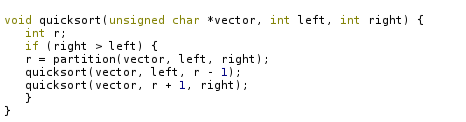
\includegraphics[width=\columnwidth]{quicksort.png}
  \caption{Quick sort implementation with recursive calls}
\end{figure}

\indent The vector that needs to be sorted has 9 elements corresponding to the current analyzed pixel of the image and its 8 neighbors. After running several tests with Quick Sort algorithm is observed that this recursive method has a high computational cost in image filtering process, requiring an extremely high processing time of about 23 miliseconds.

\subsection{Threshold}
The Threshold filter is the most simple and the fastest part of the process. It converts grayscale or color images into high contrast, black and white images. All pixels darker than 100 value are converted to black (0 value).\\
\indent Once this algorithm is based only on the verification of each image's pixel with the value of a pixel edge (which contains 100 value), the implementation must be performed using two nested loops to read all pixels, defined as an array of unsigned char terms. 

\subsection{Sobel Filter}
The Sobel Filter is normally used to image edge detection process, in order to locate the edge of an image which by finding the approximate absolute gradient magnitude at each point \textit{I} of an input grayscale image. The Sobel Filter is sensitive to noise in pictures that effectively highlight them as edges. In the presented paper a Gradient method for filter design is used: it detects the edges by looking for the maximum and minimum in the first derivative of the image. The masks presented on figure 2 are used to make all the computations, where \textit{$\mathbf{N}_{x}$} matrix is related to processing in the horizontal direction, and \textit{$\mathbf{N}_{y}$} matrix is related to the vertical direction processing.

%\centering
\begin{figure}
\[
N_{x}=\left(\begin{array}{ccc}
-1 & 0 & +1 \\
-2 & 0 & +2 \\
-1 & 0 & +1
\end{array}\right)\,\,\, N_{y}=\left(\begin{array}{ccc}
-1 & -2 & -1 \\
 0 &  0 &  0 \\
+1 & +2 & +1
\end{array}\right)
\]
\caption{Sobel filter's masks}
\end{figure}

By considering the first implementation of this method, which take into account all the elements of the matrices \textit{$\mathbf{N}_{x}$} and \textit{$\mathbf{N}_{y}$} when calculating all the values of image pixels by Sobel filtering, the time computation measured after many tests of the Sobel filter is given by \(18\) milliseconds, which is costly for image processing.

In Fig. 3. it is possible to observe the results achieved on the image of a patient with cerebral cancer, where the initial image is obtained by a MRI system without any filtering process. Thereafter a sequence of filtering is applied: Median filter, Threshold filter, and finally Sobel filter, finalizing the process of recognition of a tumor in a patient.

%%%%%%%%%%%%%%%%%%%%%%%%%%%%%%%%%%%%%%%%%%%%%%%%%%%%%%%%%%%%%%%%%%%%%%%%%%%%%
\begin{figure}[!ht]%{\linewidth}
  \centering
  %\captionsetup{justification=centering}
  
  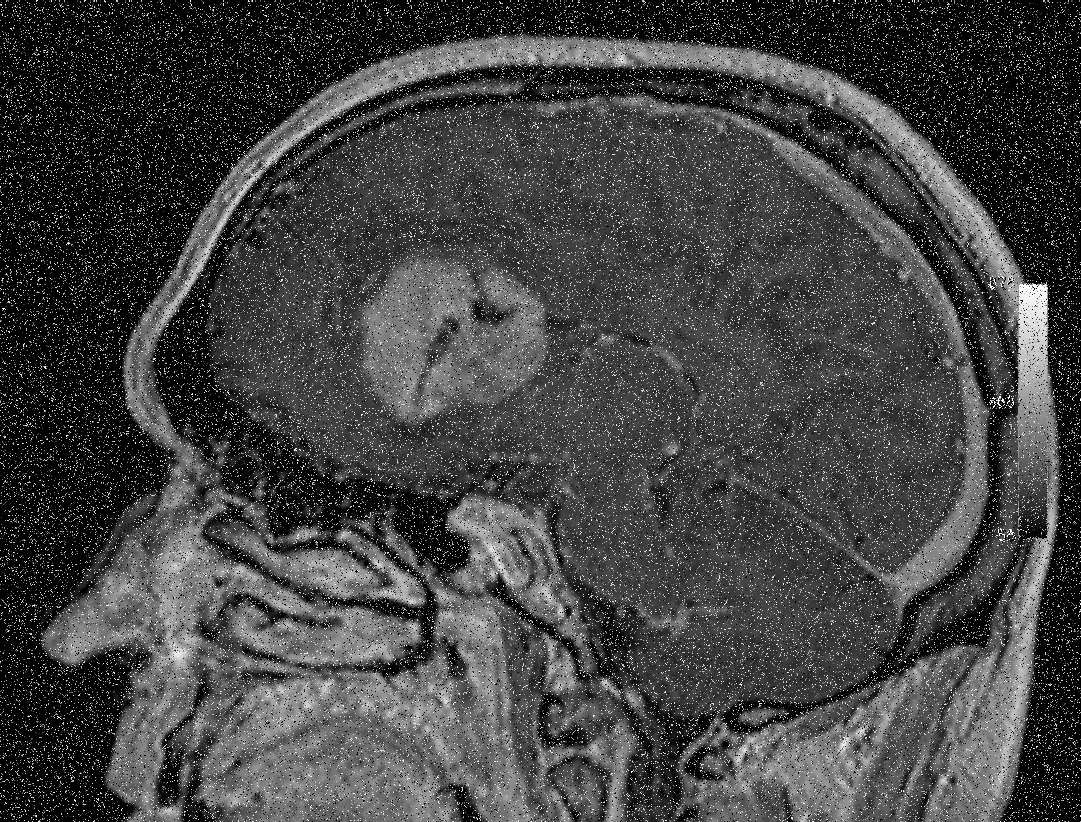
\includegraphics[scale=0.115]{cancer_noise.png}
  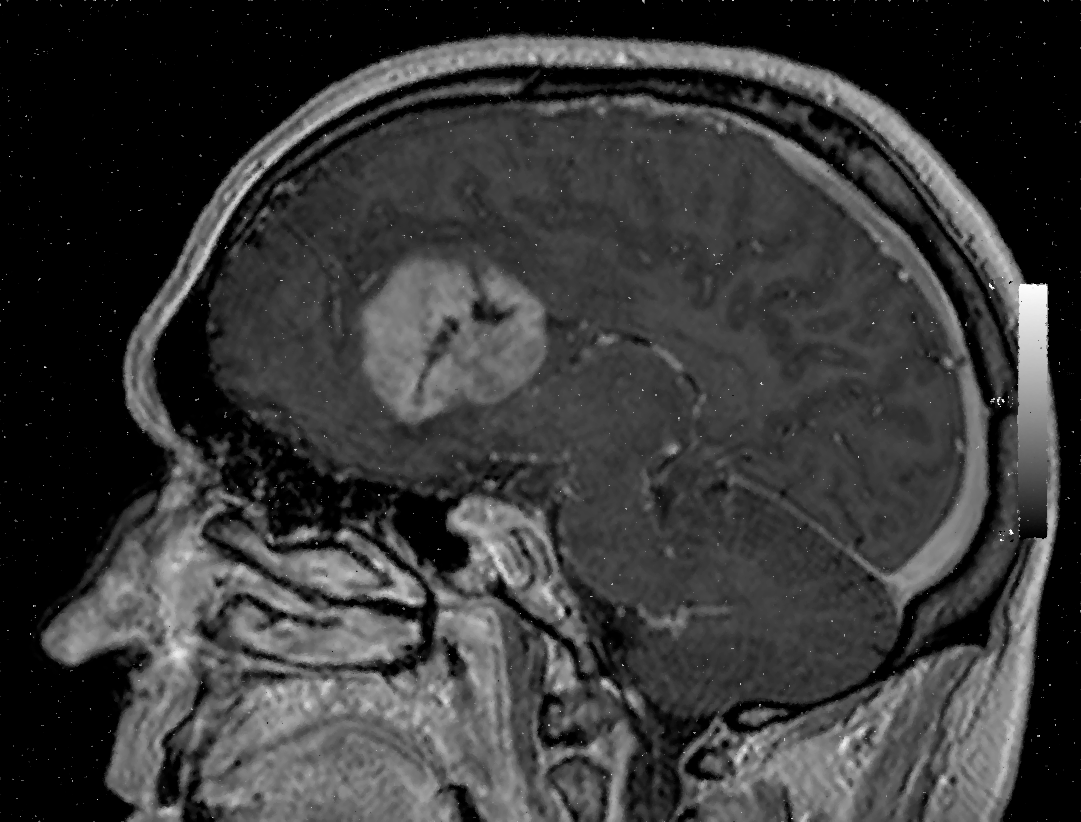
\includegraphics[scale=0.115]{cancer_noise_filtre_median.png}
  
  \par\bigskip % force a bit of vertical whitespace
  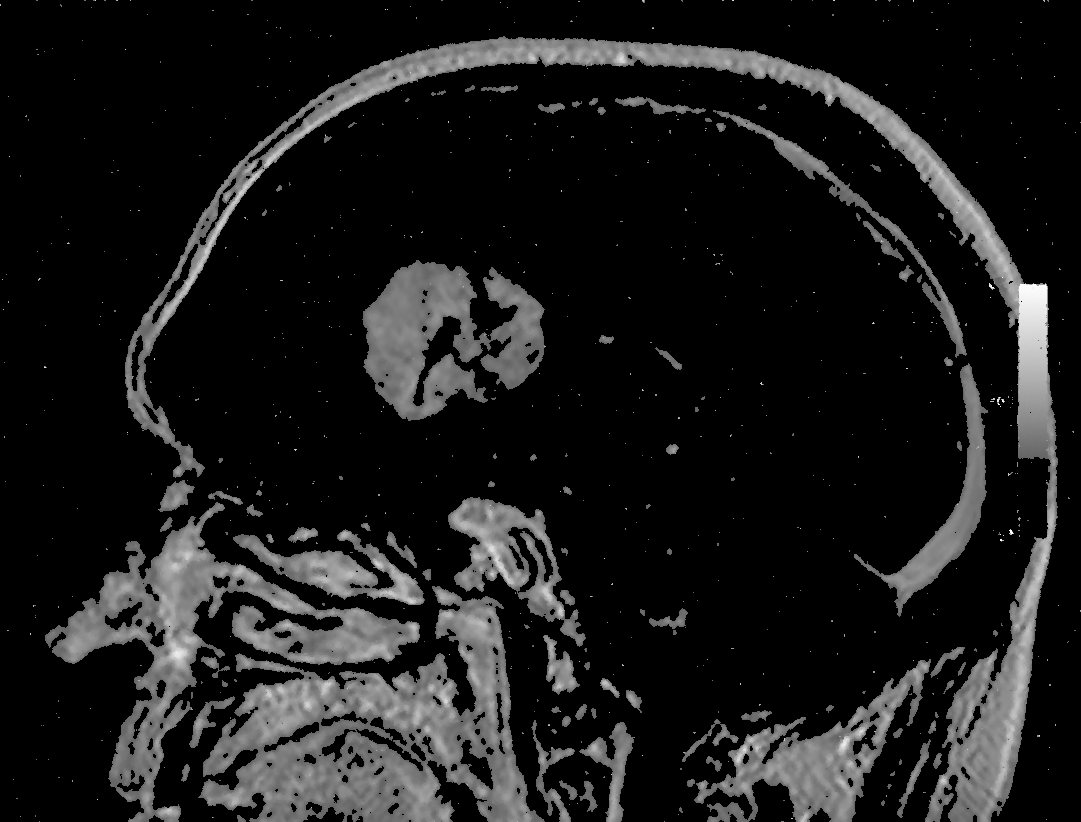
\includegraphics[scale=0.115]{cancer_noise_filtre_median_seuillage.png}
  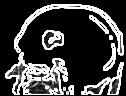
\includegraphics[scale=0.98]{results_3.jpg}
  
  \protect\caption{First the initial image obtained by MRI process is
  filtered by Median filter removing the noise in the image. After that the Threshold filter is applied in order to convert grayscale or color images into high contrast.
  Finally the Sobel filter finishes the medical image filtering process by detecting the edge of the image.}
\end{figure}
%%%%%%%%%%%%%%%%%%%%%%%%%%%%%%%%%%%%%%%%%%%%%%%%%%%%%%%%%%%%%%%%%%%%%%%%%%%%%

\section{Coding Optimisation}


From the results of computational performance obtained in a classical implementation in C language for the three analysed filters, the importance of performing optimizations must be emphasized. In this section a coding optimisation is presented in order to highlight its first impacts on image processing time filtering.


\subsection{Local Memory Use}

The default compilation of the algorithm lets the intermediate pictures on the L3 CPU cache memory which has a very high time cost access. So the first optimisation can be given by using architectures using a Generalized Shared Memory, which is maintained in a consistent state by a hardware-based coherency mechanism that operates on shared objects, wherever they happen to be calculated. In order to use this technique of memory organization the option \(LOCAL\_SHARED\) is included to the main program in order to put the data on the cash memory cluster, which is formed by one or more processors, a local main memory storing both private and shared objects and an external coherency unit connected to inter-node communication means.

After include that option, the performance dramatically improves the computational and time performance of the system, from more than \(400\) milliseconds to approximately \(40\) milliseconds for the full system, comprising the process of reading and writing, and the filtering sequence taken through Median, Threshold, and Sobel filters.

\subsection{Median Filter}

The critical part of the Median filter is the sorting algorithm. Before the optimisation phase, the system used a quick sort algorithm using recursion calls. Replacing it by an insertion sort algorithm the filtering process has improved the performances by 20\% . 

\begin{figure}[!ht]%{\linewidth}
  \centering
  \captionsetup{justification=centering}
  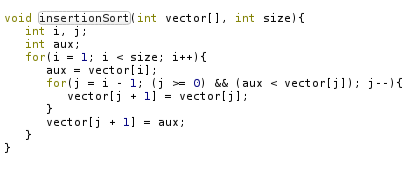
\includegraphics[width=\columnwidth]{insersionSort.png}
  \caption{Insertion sort algorithm implementation}
\end{figure}

Due to the high computational efficiency of the insertion algorithm with small lists (which depends on the computational power of the computer is running on), and the high efficiency with memory once this sorting algorithm needs one extra storage location to making room for moving elements, the insertion sort algorithm is used on Median filtering process of the image, which is the first filter used to highlight the cancer tumor in an medical image, in order to reduce the calculation time required for image processing. In other words, the insertion sort algorithm is statistically more efficient than a quick sort for 9 values, and does not use recursive calls in the sorting process.
After running several tests with Insertion Sort algorithm is observed that this method has a small computational cost in comparison with Quick Sort, requiring a smaller processing time of about 16 milliseconds on image filtering process.

\subsection{Threshold}
In order to optimise the Threshold filtering process, the loop unrolling technique, which is easily applied to sequential array processing loops where the number of interactions is known prior to execution of the loop, is used in order to improve the gains by reduction the computation of complex instructions. In other words, this technique is applied by replicating the code inside the two nested loops body 27 times (which is the loop unrolling factor), decreasing the number of interactions, and yields to increase the size of the code.

\subsection{Sobel Filter}
The Sobel Filter can be optimized by avoiding unnecessary computations, which depend of the values of \textit{$\mathbf{N}_{x}$} and \textit{$\mathbf{N}_{y}$} matrices. In the analyzed case in this paper, by considering the matrices in Fig. 2, the following considerations can be observed:


\begin{itemize}
\item The central column of \(N_x\) is empty.
\item The central line of \(N_y\) is empty.
\item Up left and bottom right values can be reused for each mask.
\item Up right and bottom left values can be reused after an reversing them.
\end{itemize}

These optimisations reduce the time computation specifically for the Sobel filter to \(1,93\) milliseconds, which represents a gain of approximately 89,4\% compared with the first implemented algorithm.

\section{Process Parallelization}

Parallel processing divides a large task into many smaller tasks and executes them concurrently on several nodes in order to computes larger tasks more quickly. In this section a process parallelization of the code is presented by using important computational tools.

\subsection{Open MP}
Open MP is a standard API that can be used in shared memory programs, which are written in C and C++. It consists of compiler directives, functions, and environment variables. In the presented paper a GNU compiler is used to create the executable code, nevertheless Open MP is supported by many other compilers, and data decomposition is handled automatically. In order to run efficiently the code written for filtering image processing, just a shared memory multiprocessor architecture is used. Thus a cluster with 8 cores is used in order to divide the image in 8 parts resulting in a faster computation of the final values of each pixel in the image.

\subsection{Performance Analysis}
Image processing is a very relevant field for using a high level of parallelization. Thanks to its eight cores, the Virtual-SoC cluster could theoretically reduce by a factor of eight the computation time. The system was strongly optimized on the threshold and mainly the Sobel Filter. The median filter still resists. However, it should be remembered that the input picture is still on the L3 memory, explaining the lack of efficiency of the parallelization. As a last resort, we suggest to use an hardware acceleration for the median filter to beat the time target.\\


\begin{tabular}[!h]{|l|c|c|r|}
  \hline
  Filter & Without OpenMP & With OpenMP & Factor \\
  \hline
  Median & 18 545 678 ns & 10 966 160 ns & 1,69 \\
  \hline
  Threshold & 240 480 ns & 57 682 ns & 4,17\\
  \hline
  Sobel & 1 928 154 ns & 437 472 ns & 4,41\\
  \hline
  Total & 20 714 312 ns & 11 461 314 ns & 1,81\\
  \hline
\end{tabular}

\section{Hardware Acceleration}

Motivated by the knowledge that hardware acceleration is a technique in which a computer’s hardware is forced to perform faster than the standard computing architecture of a normal central processing unit (CPU), the strategy implemented as well as its description are presented in this section, in order to obtain the minimal computational time cost in filtering process.

\subsection{Communication with the accelerator}

In order to use efficiently the accelerator, it is important to know how to communicate with it from the memory or the processor. The process needs to send 8-bits pixels to the accelerator and the word are 32-bits. So, each word will regroup 4 pixels, written and read on the word with shifting operators and masks. Results are shown on Fig. 4. Results point out how much it is important to process the operation from the local shared memory.

\begin{figure}[!ht]
  \centering

  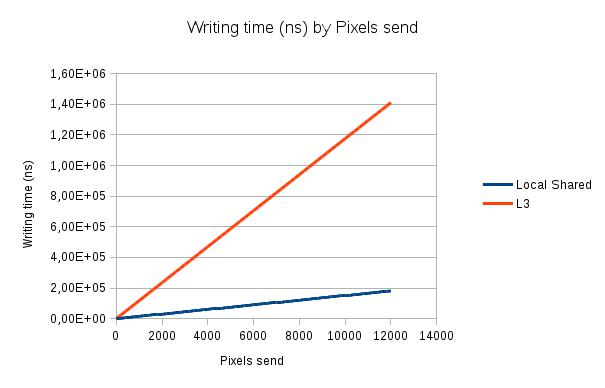
\includegraphics[scale=0.45]{graph.jpg}
  
  \protect\caption{Writing time on the accelerator form the processor, when the pixels come from the L3 or the Local Shared memory. Packaging process is included.}
\end{figure}

\subsection{Acceleration strategy}

Hardware acceleration of sorting algorithms is a complex issue with an abundant literature. However, the used system with a median filter using the eight neighbours of each pixel  could only deals with nine values. More specifically, it only looks for the median value of them and does not have to complete the sort of the array. Moreover, hardware acceleration offers the opportunity to parallelize the process and making simultaneously several comparisons.

To make the system more reliable, it is possible to only use a very stable sort algorithm. Actually it is even possible to do the process without sorting, by using a test that assess if it is the median of a vector or not. The tested value is compared to every others and the results of each comparisons are preserved. If the difference between the number of higher and smaller value is smaller than the number of values equal to the tested one, it is a median: 

\begin{math}
if \|bigger - smaller\| <= equal -> is\_median
\end{math}

\subsection{Hardware acceleration steps}

\begin{figure*}
  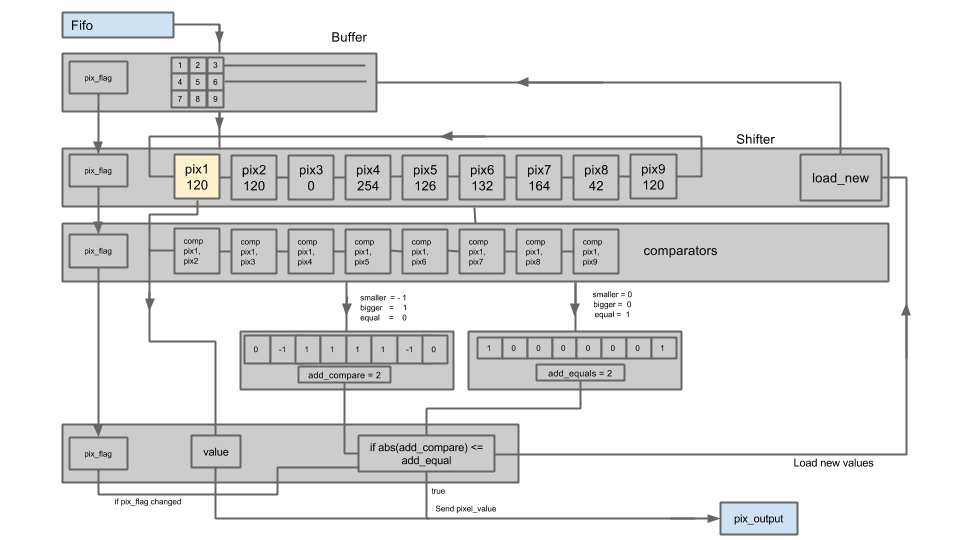
\includegraphics[width=\textwidth]{slide_sc.png}
  \caption{Diagram of the hardware accelerator. The fifo above the diagram receives four pixels at the same time from the PIC, but it sends them only one by one. It is the opposite for the output.}
\end{figure*}

The next section presents the different steps of the hardware accelerator based on this strategy. All of them can be pipe-lined:

\begin{itemize}
\item \textbf{Image buffering:} The median filter needs to work on a 3x3 area. So we will use a buffer of pixels to have a direct access to these 9 pixels at each pixel reception. Unfortunately, it increases the time process of this number of pixel reading. However it is a small value.
\item \textbf{3x3 pixels loading:} This module receives the nine pixels used for computation. It is a loop shifter.
\item \textbf{Comparators:} This module includes eight sub-modules which are 8 bits comparator with two outputs : one is a 2-bits value giving 1 if the first pixel is bigger, 0 if it is equal, -1 if it is smaller. The second output is one if the two values are equals, zero if none.
\item \textbf{Adders:} This module contains two 8 x 4 bits registers with an output giving the sum of all their respective values. The first register receive the first output of the comparators, the second one the second output.
\item \textbf{Results:} This module receives the two results of former adders. If the absolute value of the equal adder result is greater than or equal to the compare adder result, the process found the median value. The module sends it as an output. Moreover, it sends a signal to the shifter to download new values from the buffer, to start the process for the next pixel.
\end{itemize}

\subsection{Implementation}
Due to several issues from event management. Only a non pipe-lined version of the accelerator was done. It means that the shifter will wait for the acknowledgement of the result module. It will load a new set of 3x3 pixels if the result say it is an output pixel, or it will shift if it is not. Also due to event management problems, the picture will be completely loaded on the accelerator memory before the process.

The implementation was done with five threads :

\begin{itemize}
\item \textbf{Do\ shifter:} Process the shifter and initialize the process.
\item \textbf{Do\_compare:} Take the current values from the shifter and process the evaluation. The first pixel is compared to the 8 others. Results are written in two vectors, adder and equal. First tells if the pixel is bigger (1) or smaller (-1) and the second tells if the pixel is equal (1) or not(0).

\item \textbf{Do\_adder:} Add all the elements from the adder vector and return its absolute part.
\item \textbf{Do\_equal:} Add all the elements from the equal vector and return the result. It is processed at the sime time as Do\_adder.
\item \textbf{Do\_result:} It compares the results of Do\_adder and Do\_equals. If Do\_equals result is bigger, the process found a new pixel and asks the shifter to load new values.
\end{itemize}

\subsection{Expected Results}

It is possible to estimate theoretically, the time used for the new hardware median filter. The buffer can send a pixel at each clock tick. It can be assumed that the comparison process, the adding and the final step also last one clock tick each other. The worst case appears when the only median values is downloaded on the second pixel location. In this case, the loop takes \(15\) clock ticks : four for one process, plus eight process pipe-lined and three ticks for the return of the pixel flag. It equals to \(30\) nanoseconds which is more than the reading process of a pixel from the PIC. In this case, the median filter lasts \(0,36\) milliseconds which is less than the time target, assuming the Sobel filter lasts \(0,44\) milliseconds and the threshold \(0,05\) with parallelized process. However, the statistical average of points gives a number of reduce the number of loops by a half.

\subsection{Experienced Results}

Finally after the implementation of the algorithms performance improvement, the results are measured and shown in the following table:\\

\begin{tabular}[!h]{|l|r|}
  \hline
  Process & time (ns)\\
  \hline
  Writing on accelerator & 183 454\\
  \hline
  Accelerator Process & 975 996\\
  \hline
  Reading on accelerator & 194 906\\
  \hline
  Complete process & 2 294 240\\
  \hline
  Only software (Local shared input picture) & 4 111 428\\
  \hline
\end{tabular}\\ \\

The time target is not reached, but a good improvement was done. Pipelining Writing, Acceleration Process and Reading could reduce the time of the median filter under the millisecond. Moreover, the process of the accelerator can be improved by a more efficient event management.

%%%%%%%%%%%%%%%%%%%%%%%%%%%%%%%%%%%%%%%%%%%%%%%%%%%%%%%%%%%%%%%%%%%%%%%%%%%%%
%\begin{figure}
%\centering
%\captionsetup{justification=centering}
%\begin{subfigure}% {.49\textwidth}
%  \centering
%  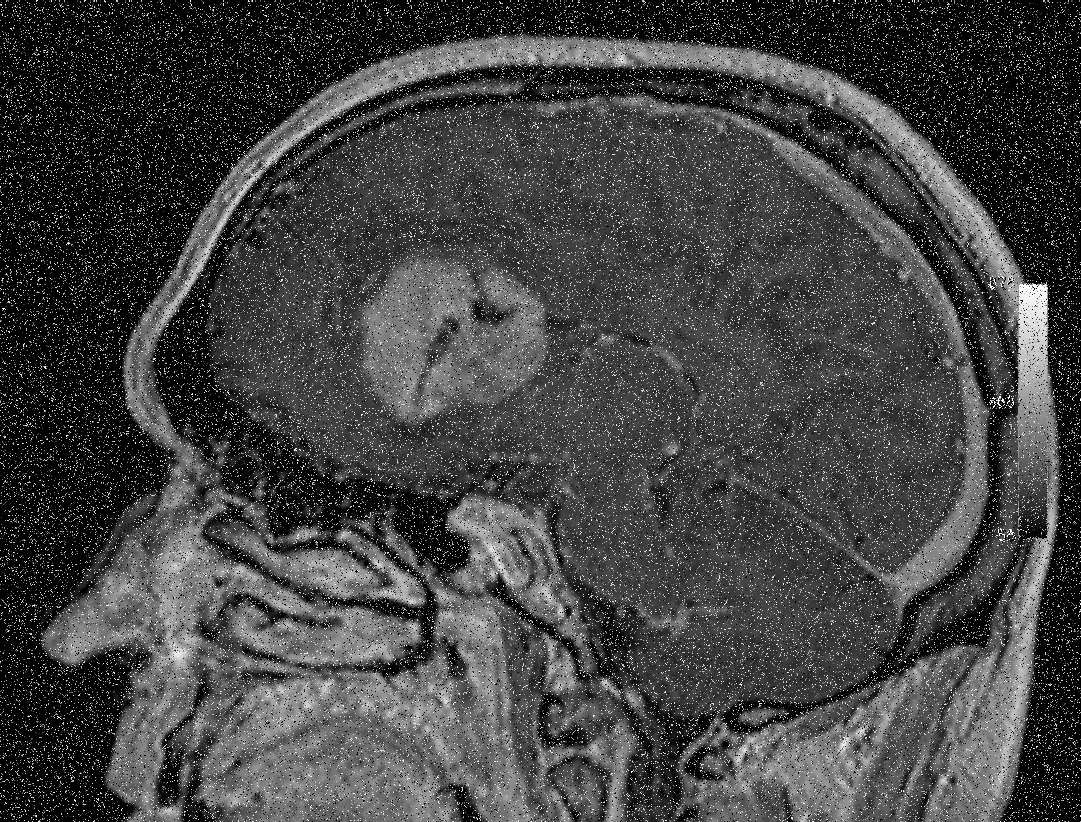
\includegraphics[scale=0.1]{cancer_noise.png}
%  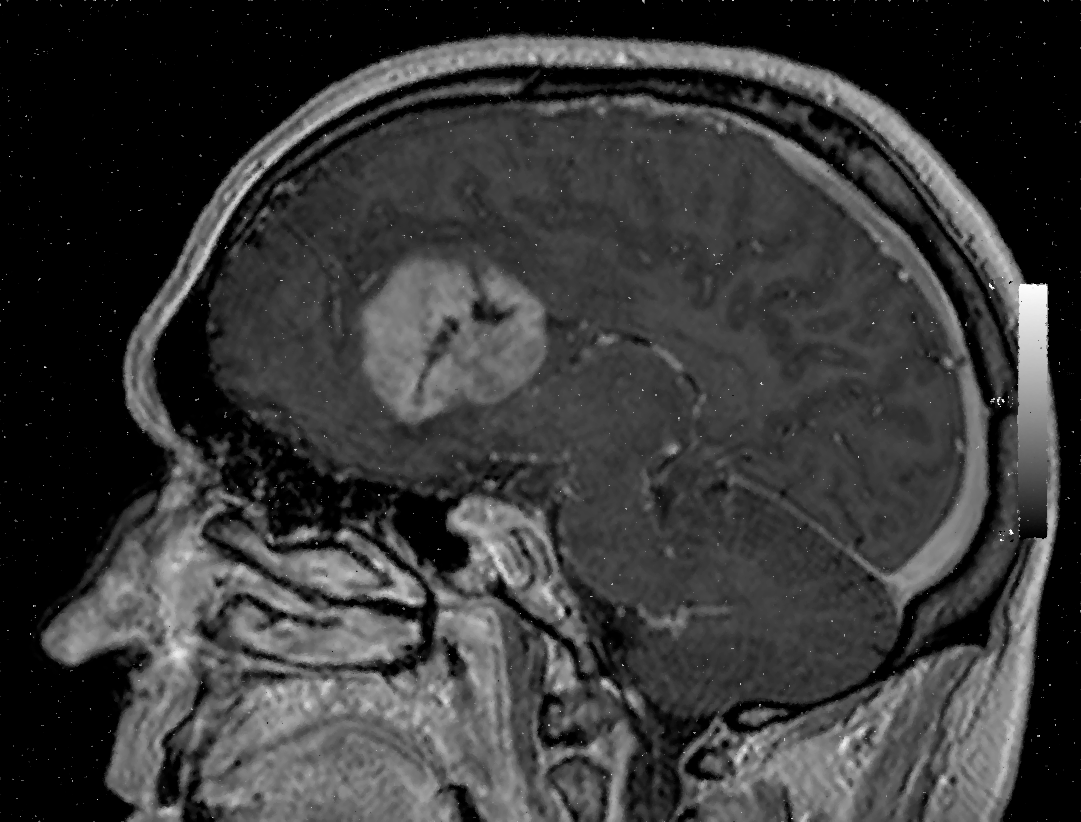
\includegraphics[scale=0.1]{cancer_noise_filtre_median.png}
%  \caption{t = 0.5 s and Re = 100}
%\end{subfigure}
%\par\bigskip % force a bit of vertical whitespace
%\begin{subfigure}% {.49\textwidth}
%   \centering
%   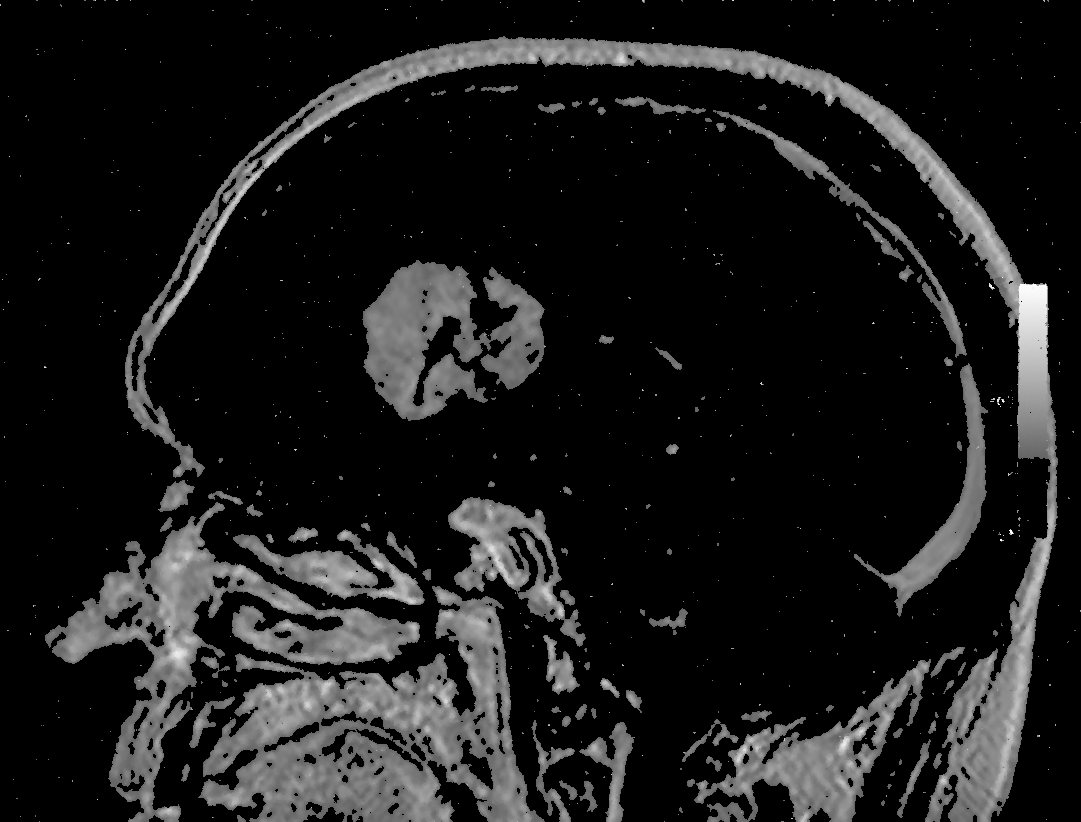
\includegraphics[scale=0.1]{cancer_noise_filtre_median_seuillage.png}
%   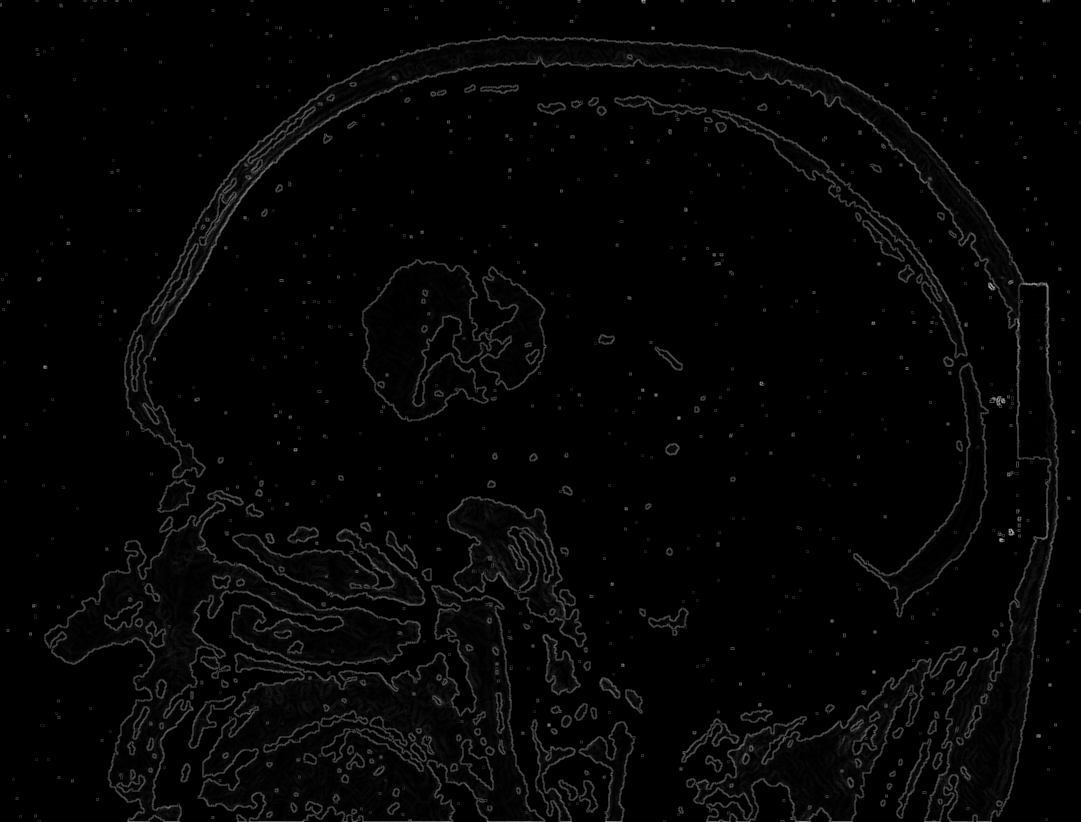
\includegraphics[scale=0.1]{cancer_noise_filtre_median_seuillage_sobel.png}
%   \caption{t = 1.0 s and Re = 200}
%\end{subfigure}
%\end{figure}
%%%%%%%%%%%%%%%%%%%%%%%%%%%%%%%%%%%%%%%%%%%%%%%%%%%%%%%%%%%%%%%%%%%%%%%%%%%%%

\section{Conclusion}

%\blindtext
The implementation of the Median, Threshold and Sobel filters normally has a high computational cost, resulting in high time filtering of images. In order to avoid that problem a software/hardware optimisation of the filtering process is used, divided in two parts. In the first part a software optimisation using Open MP and loop unrolling are made, improving the computational efficiency of Threshold and Sobel filters. In the second part the Chip Modelling (SystemC) is used in order to decrease the computational cost of Median filter, the most costly algorithm of the 3 filters chosen in this paper.

If the accelerator helped to improve the global performance of the algorithm, the time target is still not reached. However, some possible improvement are described in this paper but not implemented or tested. 

The participation of the authors in this paper, which was proposed within the context of the course SystemC at ENSTA Paristech, was at times divided into different parts between them, and at other times has made in team. Henrique VICENTE SOUZA is responsible for the first implementation process, comprising the implementation of the three algorithms (Median, Threshold and Sobel filters) in C language, which were extremely important for the initiation of the following steps, being the basis of all parts of the project. In addition He is responsible for the coding optimisation, concerning the implementation of the insertion sort in Median filter, and the loop unrolling technique in Threshold filter. After that, He did the implementation of Open MP tool, including the compiler directives, functions and environment variables in the main program. By the other hand, Alexandre LEFORT is responsible for the acceleration strategy, aiming to implement a hardware accelerator as described in Fig. \(6\)., comprising the acceleration strategy and the hardware acceleration process.

Last but not least, regarding the work made in group, it is important to highlight that throughout the process of verification and validation of all the different stages of the project there is a participation of both authors Henrique and Alexandre, as well as in the process of local memory use, the code optimisation of Sobel filter (by avoiding unnecessary computations), and the performance analysis of all the obtained results.



\appendices
%\section{Proof of the First Zonklar Equation}
%Some text for the appendix.

% use section* for acknowledgement
\section*{Acknowledgment}

This work is the result of a System on Chip Modelling (SystemC) Project at ENSTA - Paristech in Paris, France guided by Prof. Nicolas VENTROUX.

The authors would like to thank to ENSTA - Paristech for the opportunity to acquire experience in research and development, and their Prof. Nicolas VENTROUX for the guidance,  all support during all steps of the project and relevant discussions that helped the authors in the process of understanding, analysing and correcting various problems of the project.


% Can use something like this to put references on a page
% by themselves when using endfloat and the captionsoff option.
\ifCLASSOPTIONcaptionsoff
  \newpage
\fi



% trigger a \newpage just before the given reference
% number - used to balance the columns on the last page
% adjust value as needed - may need to be readjusted if
% the document is modified later
%\IEEEtriggeratref{8}
% The "triggered" command can be changed if desired:
%\IEEEtriggercmd{\enlargethispage{-5in}}

% references section

% can use a bibliography generated by BibTeX as a .bbl file
% BibTeX documentation can be easily obtained at:
% http://www.ctan.org/tex-archive/biblio/bibtex/contrib/doc/
% The IEEEtran BibTeX style support page is at:
% http://www.michaelshell.org/tex/ieeetran/bibtex/
%\bibliographystyle{IEEEtran}
% argument is your BibTeX string definitions and bibliography database(s)
%\bibliography{IEEEabrv,../bib/paper}
%
% <OR> manually copy in the resultant .bbl file
% set second argument of \begin to the number of references
% (used to reserve space for the reference number labels box)
\begin{thebibliography}{1}

%\bibitem{IEEEhowto:kopka}
%H.~Kopka and P.~W. Daly, \emph{A Guide to \LaTeX}, 3rd~ed.\hskip 1em plus
%  0.5em minus 0.4em\relax Harlow, England: Addison-Wesley, 1999.
  
\bibitem{IEEEhowto:ventroux}
N.~VENTROUX, \emph{Mod\'{e}lisation Syst\`{e}me sur Puce (SystemC)}, Polycopie ENSTA-Paristech,
%\hskip 1em plus 0.5em minus 0.4em
\relax Paris, France, 2014.

\end{thebibliography}

% biography section
% 
% If you have an EPS/PDF photo (graphicx package needed) extra braces are
% needed around the contents of the optional argument to biography to prevent
% the LaTeX parser from getting confused when it sees the complicated
% \includegraphics command within an optional argument. (You could create
% your own custom macro containing the \includegraphics command to make things
% simpler here.)
%\begin{biography}[{\includegraphics[width=1in,height=1.25in,clip,keepaspectratio]{mshell}}]{Michael Shell}
% or if you just want to reserve a space for a photo:

% You can push biographies down or up by placing
% a \vfill before or after them. The appropriate
% use of \vfill depends on what kind of text is
% on the last page and whether or not the columns
% are being equalized.

%\vfill

% Can be used to pull up biographies so that the bottom of the last one
% is flush with the other column.
%\enlargethispage{-5in}



% that's all folks
\end{document}


